\section{Auswertung}
\label{sec:Auswertung}

\subsection{Messung bis 1 bar}

Zur Berechnung der Verdampfungswärme $L$ wird die in (\ref{eq:damppfdruck}) hergeleitete Gleichung 
\begin{equation}
    \ln \left(\frac{p}{p_{0}}\right) = -\frac{L}{R} \cdot \frac{1}{T}
\end{equation}
verwendet. Der zu Beginn gemesse Umgebungsdruck beträgt dabei
\begin{equation}
    p_{0} = \qty{1013e2}{kPa} \, .
\end{equation}

\begin{table} [h!]
    \centering
    \caption{Messwerte des Drucks $p$ bis $\qty{1}{bar}$}
    \label{tab:daten1}
    \begin{tabular}{c c c c c c c c c}
        \toprule
        $T \mathbin{/} \unit{\celsius}$ & $T \mathbin{/} \unit{\kelvin}$ &  $p \mathbin{/} \unit{\milli\bar}$ & $p \mathbin{/} \unit{\kilo\pascal}$ & $\quad$ &
        $T \mathbin{/} \unit{\celsius}$ & $T \mathbin{/} \unit{\kelvin}$ &  $p \mathbin{/} \unit{\milli\bar}$ & $p \mathbin{/} \unit{\kilo\pascal}$ \\
        \midrule
        18 & 291.15 &    52 &    5.2 & $\quad$ &  56 & 329.15 &   246 &   24.6 \\
        19 & 292.15 &    81 &    8.1 & $\quad$ &  57 & 330.15 &   250 &   25.0 \\
        20 & 293.15 &    87 &    8.7 & $\quad$ &  58 & 331.15 &   258 &   25.8 \\
        21 & 294.15 &    94 &    9.4 & $\quad$ &  59 & 332.15 &   260 &   26.0 \\
        22 & 295.15 &   100 &   10.0 & $\quad$ &  60 & 333.15 &   267 &   26.7 \\
        23 & 296.15 &   104 &   10.4 & $\quad$ &  61 & 334.15 &   278 &   27.8 \\
        24 & 297.15 &   106 &   10.6 & $\quad$ &  62 & 335.15 &   285 &   28.5 \\
        25 & 298.15 &   108 &   10.8 & $\quad$ &  63 & 336.15 &   289 &   28.9 \\
        26 & 299.15 &   112 &   11.2 & $\quad$ &  64 & 337.15 &   290 &   29.0 \\
        27 & 300.15 &   117 &   11.7 & $\quad$ &  65 & 338.15 &   301 &   30.1 \\
        28 & 301.15 &   122 &   12.2 & $\quad$ &  66 & 339.15 &   317 &   31.7 \\
        29 & 302.15 &   127 &   12.7 & $\quad$ &  67 & 340.15 &   320 &   32.0 \\
        30 & 303.15 &   130 &   13.0 & $\quad$ &  68 & 341.15 &   334 &   33.4 \\
        31 & 304.15 &   136 &   13.6 & $\quad$ &  69 & 342.15 &   343 &   34.3 \\
        32 & 305.15 &   138 &   13.8 & $\quad$ &  70 & 343.15 &   350 &   35.0 \\
        33 & 306.15 &   142 &   14.2 & $\quad$ &  78 & 351.15 &   464 &   46.4 \\
        34 & 307.15 &   143 &   14.3 & $\quad$ &  79 & 352.15 &   478 &   47.8 \\
        35 & 308.15 &   146 &   14.6 & $\quad$ &  80 & 353.15 &   500 &   50.0 \\
        36 & 309.15 &   148 &   14.8 & $\quad$ &  81 & 354.15 &   528 &   52.8 \\
        37 & 310.15 &   152 &   15.2 & $\quad$ &  82 & 355.15 &   549 &   54.9 \\
        38 & 311.15 &   155 &   15.5 & $\quad$ &  83 & 356.15 &   563 &   56.3 \\
        39 & 312.15 &   160 &   16.0 & $\quad$ &  84 & 357.15 &   575 &   57.5 \\
        40 & 313.15 &   162 &   16.2 & $\quad$ &  85 & 358.15 &   599 &   59.9 \\
        41 & 314.15 &   166 &   16.6 & $\quad$ &  86 & 359.15 &   629 &   62.9 \\
        42 & 315.15 &   167 &   16.7 & $\quad$ &  87 & 360.15 &   643 &   64.3 \\
        43 & 316.15 &   173 &   17.3 & $\quad$ &  88 & 361.15 &   666 &   66.6 \\
        44 & 317.15 &   177 &   17.7 & $\quad$ &  89 & 362.15 &   696 &   69.6 \\
        45 & 318.15 &   186 &   18.6 & $\quad$ &  90 & 363.15 &   715 &   71.5 \\
        46 & 319.15 &   187 &   18.7 & $\quad$ &  91 & 364.15 &   748 &   74.8 \\
        47 & 320.15 &   195 &   19.5 & $\quad$ &  92 & 365.15 &   793 &   79.3 \\
        48 & 321.15 &   198 &   19.8 & $\quad$ &  93 & 366.15 &   809 &   80.9 \\
        49 & 322.15 &   200 &   20.0 & $\quad$ &  94 & 367.15 &   839 &   83.9 \\
        50 & 323.15 &   207 &   20.7 & $\quad$ &  95 & 368.15 &   862 &   86.2 \\
        51 & 324.15 &   216 &   21.6 & $\quad$ &  96 & 369.15 &   898 &   89.8 \\
        52 & 325.15 &   222 &   22.2 & $\quad$ &  97 & 370.15 &   919 &   91.9 \\
        53 & 326.15 &   226 &   22.6 & $\quad$ &  98 & 371.15 &   962 &   96.2 \\
        54 & 327.15 &   231 &   23.1 & $\quad$ &  99 & 372.15 &   986 &   98.6 \\
        55 & 328.15 &   238 &   23.8 & $\quad$ & 100 & 373.15 &  1016 &  101.6 \\
        \bottomrule
    \end{tabular}        
\end{table}

Aus den gemessenen Wertepaaren $(p,T)$ in \autoref{tab:daten1} und einer linearen Ausgleichsrechnung
wird mittels SCIPY \cite{scipy} die Ausgleichsgerade der Form
\begin{equation}
    y = ax + b 
\end{equation}
in Abbildung \ref{fig:plot1} dargestellt.
Es sei angemerkt, dass aufgrund von Problemen bei der Messung einige Daten nicht aufgezeichnet wurden,
was die Lücke bei der Messreihe erklärt.
\begin{figure}[H]
    \centering
    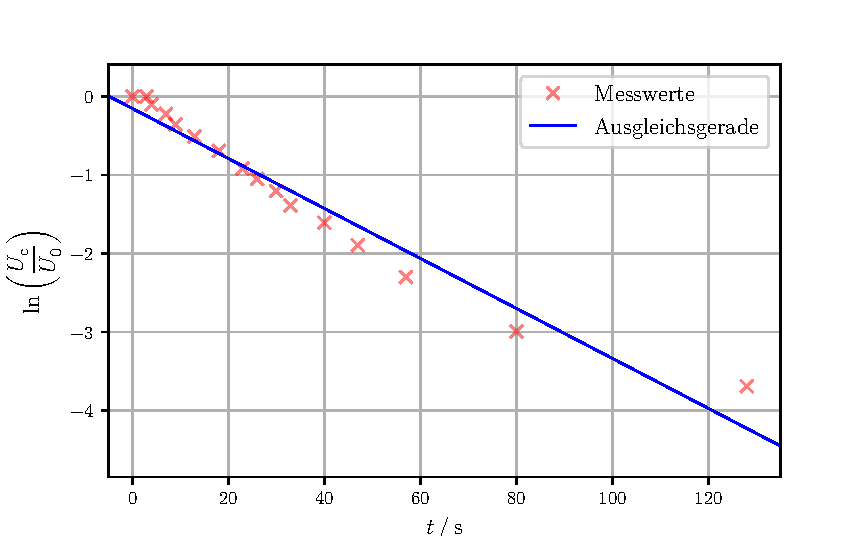
\includegraphics[width=\textwidth]{plot1.pdf}
    \caption{Ausgleichsgerade im Druckbereich $p \leq \qty{1}{bar}$.}
    \label{fig:plot1}
\end{figure}

Für die Parameter ergeben sich somit
\begin{align*}
    a &= \num{-3.225(060)e3} \quad \text{und} \\
    b &= \num{15.38(17)} \, .
\end{align*}

Wird die Beziehung der Steigung $a$ aus (\ref{eq:damppfdruck}) verwendet, lässt sich $L$ damit durch
\begin{equation}
    a = -\frac{L}{R} \quad \Rightarrow \quad L=-a \cdot R
\end{equation}
ausdrücken. 
Somit ergibt sich die Verdampfungswärme zu
\begin{equation}
    L = \qty{26.8(5)}{\kilo\joule\per\mol} \, .
\end{equation}

Die äußere Verdampfungswärme $L_\text{a}$ ist die benötigte Energie, 
um das Volumen eines Mols der Flüssigkeit auf das Volumen eines Mols des Gases zu vergrößern.
Wird die dabei verrichtete Volumenarbeit $W = pV$  gleich der idealen Gasgleichung (\ref{eq:idgasgleichung})
gesetzt, ergibt sich bei $T = \qty{373}{K}$ für die äußere Verdampfungswärme
\begin{equation}
    L_{\text{a}} = W = pV = RT = \qty{3.101}{\kilo\joule\per\mol} \text{ .}
\end{equation}

Die benötigte innere Energie $L_\text{i}$ um die molekularen Bindungskräfte bei der Verdampfung zu überwinden ist damit
\begin{equation}
    L_{\mathrm{i}} = L-L_{\mathrm{a}} = \qty{23.7(5)}{\kilo\joule\per\mol} \, .
\end{equation}

Eine Division durch die Avogadro-Konstante $N_\text{A} = \qty{6.022e23}{\per\mol}$
ergibt die innere Energie pro Molekül. Somit lautet das Ergebnis in Elektronenvolt
\begin{equation}
    L_{\text{i}} = \qty{0.246(5)}{\eV} \, .
\end{equation}


\subsection{Messung von 1 bis 15 bar}

\begin{table} [h]
    \centering
    \caption{Messwerte des Drucks im Bereich $p \in [1, 15] \, \mathrm{bar}$}
    \label{tab:daten2}
    \begin{tabular}{c c c c}
        \toprule
        $T \mathbin{/} \unit{\celsius}$ & $T \mathbin{/} \unit{\kelvin}$ &  $p \mathbin{/} \unit{\bar}$ & $p \mathbin{/} \unit{\kilo\pascal}$ \\
        \midrule
        118 & 391.15 &    1 &  100 \\
        130 & 403.15 &    2 &  200 \\
        141 & 414.15 &    3 &  300 \\
        148 & 421.15 &    4 &  400 \\
        155 & 428.15 &    5 &  500 \\
        161 & 434.15 &    6 &  600 \\
        166 & 439.15 &    7 &  700 \\
        171 & 444.15 &    8 &  800 \\
        176 & 449.15 &    9 &  900 \\
        181 & 454.15 &   10 & 1000 \\
        184 & 457.15 &   11 & 1100 \\
        188 & 461.15 &   12 & 1200 \\
        191 & 464.15 &   13 & 1300 \\
        193 & 466.15 &   14 & 1400 \\
        197 & 470.15 &   15 & 1500 \\
        \bottomrule
        \end{tabular}
\end{table}

Mithilfe der Messdaten in \autoref{tab:daten2} soll nun die Temperaturabhängigkeit
der Verdampfungswärme $L$ untersucht werden. Dafür wird (\ref{eq:clausius}) nach $L$ umgestellt. Es gilt
\begin{equation}
    L = T \left(V_{\text{D}} - V_{\text{F}}\right) \frac {\dif{p}} {\dif{T}} \, . \label{eq:verdampfungswärme}
\end{equation}

Obwohl $V_\text{F}$ weiterhin vernachlässigbar ist, kann $V_\text{D}$ nicht mehr durch (\ref{eq:idgasgleichung})
ausgedrückt werden.
Eine bessere Näherung stellt die Gleichung
\begin{equation}
    \left(p + \frac {A} {V_{\text{D}}^{2}}\right) V_{\text{D}} = RT 
    \quad \text { mit } \quad
    A = \qty[per-mode=fraction]{0.9}{\joule\m\cubed\per\mol\squared} 
\end{equation}
\begin{equation}
    \Rightarrow \quad V_{\text{D}} = \frac{RT}{2p} \pm \sqrt{ \frac {R^{2} T^{2}} {4 p^{2}} - \frac{A}{p} } 
\end{equation}
dar. Somit ergibt sich für (\ref{eq:verdampfungswärme}) 
\begin{equation}
    L = T\left[\frac{R T}{2 p} \pm \sqrt{\frac{R^{2} T^{2}}{4 p^{2}}-\frac{A}{p}}\right] \frac{\dif{p}}{\dif{T}} 
    = \frac{T}{p} \left[\frac{R T}{2} \pm \sqrt{\left(\frac{R T}{2}\right)^{2}-A p}\right] \frac{\dif{p}}{\dif{T}} \, .
    \label{eq:L}
\end{equation}

Um den auftretenden Differentialquotienten $\frac{\dif{p}}{\dif{T}}$ zu bestimmen,
wird aus den gemessenen Wertepaaren $(p,T)$ ein Ausgleichsploynom 3. Grades der Form
\begin{align*}
    p(T) &= a \cdot T^{3} + b \cdot T^{2} + c \cdot T+d \quad \text{bzw.} \\
    \frac{\dif{p}}{\dif{T}} &= 3a \cdot T^{2} + 2b \cdot T + c \quad 
\end{align*}
in Abbildung \ref{fig:plot2} dargestellt.
\begin{figure}[H]
    \centering
    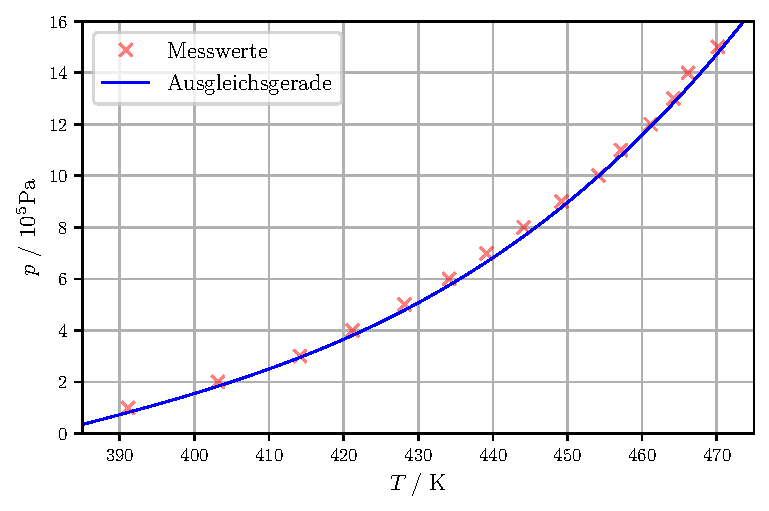
\includegraphics[width=\textwidth]{plot2.pdf}
    \caption{Ausgleichspolynom im Druckbereich $p \in [1, 15] \, \mathrm{bar}$.}
    \label{fig:plot2}
\end{figure}

Damit ergibt sich für die Parameter
\begin{align*}
    a &= \qty{1.108(341)}{\pascal\per\cubic\kelvin} \, , \\
    b &= \qty{-1.263(442)e3}{\pascal\per\kelvin\squared} \, , \\ % *10**3
    c &= \qty{4.877(1.903)e5}{\pascal\per\kelvin} \, \, \text{und} \\ % *10**5
    d &= \qty{-6.367(2.727)e7}{\pascal} \, . % *10**7
\end{align*}

Werden nun $p(T)$ und $\frac{\dif{p}}{\dif{T}}$ in \ref{eq:L} eingesetzt, 
ergibt sich die Gleichung 
\begin{align}
    L(T) &= \frac{T \left(3 a T^{2}+2 b T+c\right)}{a T^{3}+b T^{2}+c T+d} \left[\frac{R T}{2} \pm \sqrt{\left(\frac{R T}{2}\right)^{2}-A \left(a T^{3}+b T^{2}+c T+d\right)}\right]  \\
    &= \frac{3 a T^{3}+2 b T^{2}+c T}{a T^{3}+b T^{2}+c T+d} \left[\frac{R T}{2} \pm \sqrt{\left(\frac{R T}{2}\right)^{2}-A\left(a T^{3}+b T^{2}+c T+d\right)}\right] \text{ .}
\end{align}

Die daraus resultierenden temperaturabhängigen Verdampfungswärmen sind in den Abbildungen
\ref{fig:plot3} und \ref{fig:plot4} aufgetragen.

\begin{figure}[H]
    \centering
    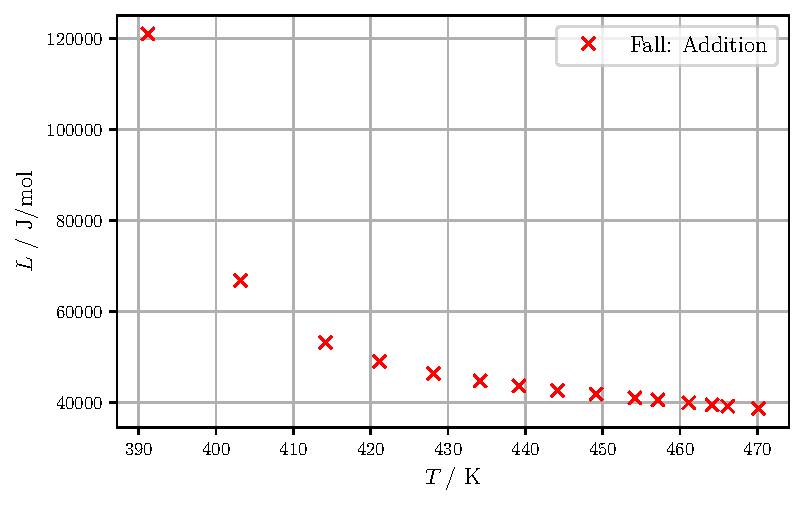
\includegraphics[width=0.9\textwidth]{plot3.pdf}
    \caption{Temperaturabhängigkeit der Verdampfungswärme im Falle der Addition.}
    \label{fig:plot3}
\end{figure}

\begin{figure}[H]
    \centering
    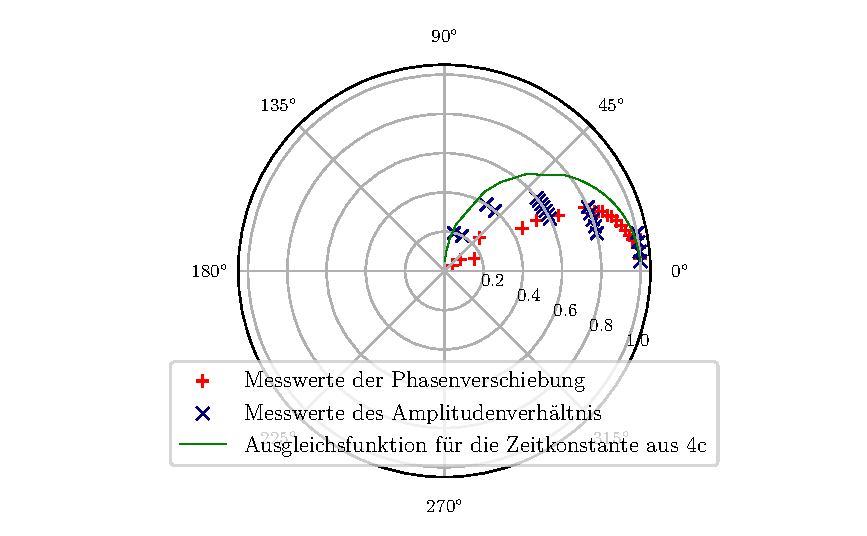
\includegraphics[width=0.9\textwidth]{plot4.pdf}
    \caption{Temperaturabhängigkeit der Verdampfungswärme im Falle der Subtraktion.}
    \label{fig:plot4}
\end{figure}